\documentclass[1p]{elsarticle_modified}
%\bibliographystyle{elsarticle-num}

%\usepackage[colorlinks]{hyperref}
%\usepackage{abbrmath_seonhwa} %\Abb, \Ascr, \Acal ,\Abf, \Afrak
\usepackage{amsfonts}
\usepackage{amssymb}
\usepackage{amsmath}
\usepackage{amsthm}
\usepackage{scalefnt}
\usepackage{amsbsy}
\usepackage{kotex}
\usepackage{caption}
\usepackage{subfig}
\usepackage{color}
\usepackage{graphicx}
\usepackage{xcolor} %% white, black, red, green, blue, cyan, magenta, yellow
\usepackage{float}
\usepackage{setspace}
\usepackage{hyperref}

\usepackage{tikz}
\usetikzlibrary{arrows}

\usepackage{multirow}
\usepackage{array} % fixed length table
\usepackage{hhline}

%%%%%%%%%%%%%%%%%%%%%
\makeatletter
\renewcommand*\env@matrix[1][\arraystretch]{%
	\edef\arraystretch{#1}%
	\hskip -\arraycolsep
	\let\@ifnextchar\new@ifnextchar
	\array{*\c@MaxMatrixCols c}}
\makeatother %https://tex.stackexchange.com/questions/14071/how-can-i-increase-the-line-spacing-in-a-matrix
%%%%%%%%%%%%%%%

\usepackage[normalem]{ulem}

\newcommand{\msout}[1]{\ifmmode\text{\sout{\ensuremath{#1}}}\else\sout{#1}\fi}
%SOURCE: \msout is \stkout macro in https://tex.stackexchange.com/questions/20609/strikeout-in-math-mode

\newcommand{\cancel}[1]{
	\ifmmode
	{\color{red}\msout{#1}}
	\else
	{\color{red}\sout{#1}}
	\fi
}

\newcommand{\add}[1]{
	{\color{blue}\uwave{#1}}
}

\newcommand{\replace}[2]{
	\ifmmode
	{\color{red}\msout{#1}}{\color{blue}\uwave{#2}}
	\else
	{\color{red}\sout{#1}}{\color{blue}\uwave{#2}}
	\fi
}

\newcommand{\Sol}{\mathcal{S}} %segment
\newcommand{\D}{D} %diagram
\newcommand{\A}{\mathcal{A}} %arc


%%%%%%%%%%%%%%%%%%%%%%%%%%%%%5 test

\def\sl{\operatorname{\textup{SL}}(2,\Cbb)}
\def\psl{\operatorname{\textup{PSL}}(2,\Cbb)}
\def\quan{\mkern 1mu \triangleright \mkern 1mu}

\theoremstyle{definition}
\newtheorem{thm}{Theorem}[section]
\newtheorem{prop}[thm]{Proposition}
\newtheorem{lem}[thm]{Lemma}
\newtheorem{ques}[thm]{Question}
\newtheorem{cor}[thm]{Corollary}
\newtheorem{defn}[thm]{Definition}
\newtheorem{exam}[thm]{Example}
\newtheorem{rmk}[thm]{Remark}
\newtheorem{alg}[thm]{Algorithm}

\newcommand{\I}{\sqrt{-1}}
\begin{document}

%\begin{frontmatter}
%
%\title{Boundary parabolic representations of knots up to 8 crossings}
%
%%% Group authors per affiliation:
%\author{Yunhi Cho} 
%\address{Department of Mathematics, University of Seoul, Seoul, Korea}
%\ead{yhcho@uos.ac.kr}
%
%
%\author{Seonhwa Kim} %\fnref{s_kim}}
%\address{Center for Geometry and Physics, Institute for Basic Science, Pohang, 37673, Korea}
%\ead{ryeona17@ibs.re.kr}
%
%\author{Hyuk Kim}
%\address{Department of Mathematical Sciences, Seoul National University, Seoul 08826, Korea}
%\ead{hyukkim@snu.ac.kr}
%
%\author{Seokbeom Yoon}
%\address{Department of Mathematical Sciences, Seoul National University, Seoul, 08826,  Korea}
%\ead{sbyoon15@snu.ac.kr}
%
%\begin{abstract}
%We find all boundary parabolic representation of knots up to 8 crossings.
%
%\end{abstract}
%\begin{keyword}
%    \MSC[2010] 57M25 
%\end{keyword}
%
%\end{frontmatter}

%\linenumbers
%\tableofcontents
%
\newcommand\colored[1]{\textcolor{white}{\rule[-0.35ex]{0.8em}{1.4ex}}\kern-0.8em\color{red} #1}%
%\newcommand\colored[1]{\textcolor{white}{ #1}\kern-2.17ex	\textcolor{white}{ #1}\kern-1.81ex	\textcolor{white}{ #1}\kern-2.15ex\color{red}#1	}

{\Large $\underline{12a_{0403}~(K12a_{0403})}$}

\setlength{\tabcolsep}{10pt}
\renewcommand{\arraystretch}{1.6}
\vspace{1cm}\begin{tabular}{m{100pt}>{\centering\arraybackslash}m{274pt}}
\multirow{5}{120pt}{
	\centering
	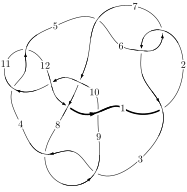
\includegraphics[width=112pt]{../../../GIT/diagram.site/Diagrams/png/1204_12a_0403.png}\\
\ \ \ A knot diagram\footnotemark}&
\allowdisplaybreaks
\textbf{Linearized knot diagam} \\
\cline{2-2}
 &
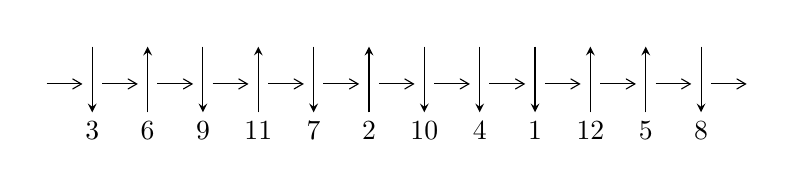
\begin{tikzpicture}[x=20pt, y=17pt]
	% nodes
	\node (C0) at (0, 0) {};
	\node (C1) at (1, 0) {};
	\node (C1U) at (1, +1) {};
	\node (C1D) at (1, -1) {3};

	\node (C2) at (2, 0) {};
	\node (C2U) at (2, +1) {};
	\node (C2D) at (2, -1) {6};

	\node (C3) at (3, 0) {};
	\node (C3U) at (3, +1) {};
	\node (C3D) at (3, -1) {9};

	\node (C4) at (4, 0) {};
	\node (C4U) at (4, +1) {};
	\node (C4D) at (4, -1) {11};

	\node (C5) at (5, 0) {};
	\node (C5U) at (5, +1) {};
	\node (C5D) at (5, -1) {7};

	\node (C6) at (6, 0) {};
	\node (C6U) at (6, +1) {};
	\node (C6D) at (6, -1) {2};

	\node (C7) at (7, 0) {};
	\node (C7U) at (7, +1) {};
	\node (C7D) at (7, -1) {10};

	\node (C8) at (8, 0) {};
	\node (C8U) at (8, +1) {};
	\node (C8D) at (8, -1) {4};

	\node (C9) at (9, 0) {};
	\node (C9U) at (9, +1) {};
	\node (C9D) at (9, -1) {1};

	\node (C10) at (10, 0) {};
	\node (C10U) at (10, +1) {};
	\node (C10D) at (10, -1) {12};

	\node (C11) at (11, 0) {};
	\node (C11U) at (11, +1) {};
	\node (C11D) at (11, -1) {5};

	\node (C12) at (12, 0) {};
	\node (C12U) at (12, +1) {};
	\node (C12D) at (12, -1) {8};
	\node (C13) at (13, 0) {};

	% arrows
	\draw[->,>={angle 60}]
	(C0) edge (C1) (C1) edge (C2) (C2) edge (C3) (C3) edge (C4) (C4) edge (C5) (C5) edge (C6) (C6) edge (C7) (C7) edge (C8) (C8) edge (C9) (C9) edge (C10) (C10) edge (C11) (C11) edge (C12) (C12) edge (C13) ;	\draw[->,>=stealth]
	(C1U) edge (C1D) (C2D) edge (C2U) (C3U) edge (C3D) (C4D) edge (C4U) (C5U) edge (C5D) (C6D) edge (C6U) (C7U) edge (C7D) (C8U) edge (C8D) (C9U) edge (C9D) (C10D) edge (C10U) (C11D) edge (C11U) (C12U) edge (C12D) ;
	\end{tikzpicture} \\
\hhline{~~} \\& 
\textbf{Solving Sequence} \\ \cline{2-2} 
 &
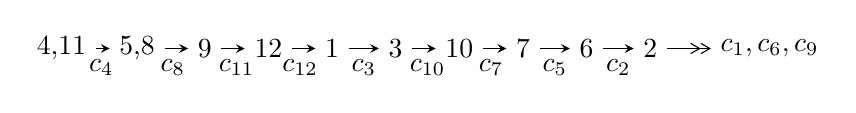
\begin{tikzpicture}[x=23pt, y=7pt]
	% node
	\node (A0) at (-1/8, 0) {4,11};
	\node (A1) at (17/16, 0) {5,8};
	\node (A2) at (17/8, 0) {9};
	\node (A3) at (25/8, 0) {12};
	\node (A4) at (33/8, 0) {1};
	\node (A5) at (41/8, 0) {3};
	\node (A6) at (49/8, 0) {10};
	\node (A7) at (57/8, 0) {7};
	\node (A8) at (65/8, 0) {6};
	\node (A9) at (73/8, 0) {2};
	\node (C1) at (1/2, -1) {$c_{4}$};
	\node (C2) at (13/8, -1) {$c_{8}$};
	\node (C3) at (21/8, -1) {$c_{11}$};
	\node (C4) at (29/8, -1) {$c_{12}$};
	\node (C5) at (37/8, -1) {$c_{3}$};
	\node (C6) at (45/8, -1) {$c_{10}$};
	\node (C7) at (53/8, -1) {$c_{7}$};
	\node (C8) at (61/8, -1) {$c_{5}$};
	\node (C9) at (69/8, -1) {$c_{2}$};
	\node (A10) at (11, 0) {$c_{1},c_{6},c_{9}$};

	% edge
	\draw[->,>=stealth]	
	(A0) edge (A1) (A1) edge (A2) (A2) edge (A3) (A3) edge (A4) (A4) edge (A5) (A5) edge (A6) (A6) edge (A7) (A7) edge (A8) (A8) edge (A9) ;
	\draw[->>,>={angle 60}]	
	(A9) edge (A10);
\end{tikzpicture} \\ 

\end{tabular} \\

\footnotetext{
The image of knot diagram is generated by the software ``\textbf{Draw programme}" developed by Andrew Bartholomew(\url{http://www.layer8.co.uk/maths/draw/index.htm\#Running-draw}), where we modified some parts for our purpose(\url{https://github.com/CATsTAILs/LinksPainter}).
}\phantom \\ \newline 
\centering \textbf{Ideals for irreducible components\footnotemark of $X_{\text{par}}$} 
 
\begin{align*}
I^u_{1}&=\langle 
-1.61209\times10^{254} u^{129}-2.93112\times10^{253} u^{128}+\cdots+1.53311\times10^{253} b-1.71265\times10^{254},\\
\phantom{I^u_{1}}&\phantom{= \langle  }-6.10829\times10^{254} u^{129}-1.85917\times10^{254} u^{128}+\cdots+1.53311\times10^{253} a-8.27337\times10^{254},\\
\phantom{I^u_{1}}&\phantom{= \langle  }u^{130}+u^{129}+\cdots-9 u^2+1\rangle \\
I^u_{2}&=\langle 
- u^{25}+6 u^{23}+\cdots-2 u^2+b,\;-6 u^{25}+36 u^{23}+\cdots+a-2,\;u^{26}-7 u^{24}+\cdots-2 u+1\rangle \\
\\
\end{align*}
\raggedright * 2 irreducible components of $\dim_{\mathbb{C}}=0$, with total 156 representations.\\
\footnotetext{All coefficients of polynomials are rational numbers. But the coefficients are sometimes approximated in decimal forms when there is not enough margin.}
\newpage
\renewcommand{\arraystretch}{1}
\centering \section*{I. $I^u_{1}= \langle -1.61\times10^{254} u^{129}-2.93\times10^{253} u^{128}+\cdots+1.53\times10^{253} b-1.71\times10^{254},\;-6.11\times10^{254} u^{129}-1.86\times10^{254} u^{128}+\cdots+1.53\times10^{253} a-8.27\times10^{254},\;u^{130}+u^{129}+\cdots-9 u^2+1 \rangle$}
\flushleft \textbf{(i) Arc colorings}\\
\begin{tabular}{m{7pt} m{180pt} m{7pt} m{180pt} }
\flushright $a_{4}=$&$\begin{pmatrix}1\\0\end{pmatrix}$ \\
\flushright $a_{11}=$&$\begin{pmatrix}0\\u\end{pmatrix}$ \\
\flushright $a_{5}=$&$\begin{pmatrix}1\\- u^2\end{pmatrix}$ \\
\flushright $a_{8}=$&$\begin{pmatrix}39.8424 u^{129}+12.1268 u^{128}+\cdots-71.6792 u+53.9645\\10.5152 u^{129}+1.91187 u^{128}+\cdots-19.4022 u+11.1711\end{pmatrix}$ \\
\flushright $a_{9}=$&$\begin{pmatrix}29.3273 u^{129}+10.2149 u^{128}+\cdots-52.2770 u+42.7935\\10.5152 u^{129}+1.91187 u^{128}+\cdots-19.4022 u+11.1711\end{pmatrix}$ \\
\flushright $a_{12}=$&$\begin{pmatrix}u\\- u^3+u\end{pmatrix}$ \\
\flushright $a_{1}=$&$\begin{pmatrix}14.5228 u^{129}+3.05728 u^{128}+\cdots-20.5663 u+22.8793\\2.96961 u^{129}-0.00148500 u^{128}+\cdots-0.904318 u+1.33697\end{pmatrix}$ \\
\flushright $a_{3}=$&$\begin{pmatrix}11.2281 u^{129}+6.52844 u^{128}+\cdots-48.1159 u+19.9734\\22.1475 u^{129}+5.96944 u^{128}+\cdots-36.2059 u+29.8117\end{pmatrix}$ \\
\flushright $a_{10}=$&$\begin{pmatrix}- u^3\\u^5- u^3+u\end{pmatrix}$ \\
\flushright $a_{7}=$&$\begin{pmatrix}47.7274 u^{129}+14.7604 u^{128}+\cdots-89.6195 u+65.9458\\-3.06650 u^{129}-2.28554 u^{128}+\cdots+5.85600 u-7.67098\end{pmatrix}$ \\
\flushright $a_{6}=$&$\begin{pmatrix}-24.2358 u^{129}-12.7252 u^{128}+\cdots+81.9825 u-40.8265\\-19.2228 u^{129}-3.74986 u^{128}+\cdots+25.3360 u-23.6219\end{pmatrix}$ \\
\flushright $a_{2}=$&$\begin{pmatrix}-55.0363 u^{129}-15.5769 u^{128}+\cdots+89.7412 u-73.3056\\11.3693 u^{129}+6.04628 u^{128}+\cdots-21.2891 u+20.2649\end{pmatrix}$\\&\end{tabular}
\flushleft \textbf{(ii) Obstruction class $= -1$}\\~\\
\flushleft \textbf{(iii) Cusp Shapes $= -71.0846 u^{129}-21.4994 u^{128}+\cdots+150.345 u-94.8308$}\\~\\
\newpage\renewcommand{\arraystretch}{1}
\flushleft \textbf{(iv) u-Polynomials at the component}\newline \\
\begin{tabular}{m{50pt}|m{274pt}}
Crossings & \hspace{64pt}u-Polynomials at each crossing \\
\hline $$\begin{aligned}c_{1},c_{5}\end{aligned}$$&$\begin{aligned}
&u^{130}+40 u^{129}+\cdots+5243 u+361
\end{aligned}$\\
\hline $$\begin{aligned}c_{2},c_{6}\end{aligned}$$&$\begin{aligned}
&u^{130}-2 u^{129}+\cdots+37 u+19
\end{aligned}$\\
\hline $$\begin{aligned}c_{3},c_{8}\end{aligned}$$&$\begin{aligned}
&u^{130}+u^{129}+\cdots+35584 u+5216
\end{aligned}$\\
\hline $$\begin{aligned}c_{4},c_{11}\end{aligned}$$&$\begin{aligned}
&u^{130}+u^{129}+\cdots-9 u^2+1
\end{aligned}$\\
\hline $$\begin{aligned}c_{7}\end{aligned}$$&$\begin{aligned}
&u^{130}-21 u^{129}+\cdots-17072 u+911
\end{aligned}$\\
\hline $$\begin{aligned}c_{9}\end{aligned}$$&$\begin{aligned}
&u^{130}-11 u^{129}+\cdots-29278734 u+4023961
\end{aligned}$\\
\hline $$\begin{aligned}c_{10}\end{aligned}$$&$\begin{aligned}
&u^{130}-61 u^{129}+\cdots-18 u+1
\end{aligned}$\\
\hline $$\begin{aligned}c_{12}\end{aligned}$$&$\begin{aligned}
&u^{130}+3 u^{129}+\cdots-44 u+1
\end{aligned}$\\
\hline
\end{tabular}\\~\\
\newpage\renewcommand{\arraystretch}{1}
\flushleft \textbf{(v) Riley Polynomials at the component}\newline \\
\begin{tabular}{m{50pt}|m{274pt}}
Crossings & \hspace{64pt}Riley Polynomials at each crossing \\
\hline $$\begin{aligned}c_{1},c_{5}\end{aligned}$$&$\begin{aligned}
&y^{130}+112 y^{129}+\cdots-2411101 y+130321
\end{aligned}$\\
\hline $$\begin{aligned}c_{2},c_{6}\end{aligned}$$&$\begin{aligned}
&y^{130}+40 y^{129}+\cdots+5243 y+361
\end{aligned}$\\
\hline $$\begin{aligned}c_{3},c_{8}\end{aligned}$$&$\begin{aligned}
&y^{130}+105 y^{129}+\cdots+1506854912 y+27206656
\end{aligned}$\\
\hline $$\begin{aligned}c_{4},c_{11}\end{aligned}$$&$\begin{aligned}
&y^{130}-61 y^{129}+\cdots-18 y+1
\end{aligned}$\\
\hline $$\begin{aligned}c_{7}\end{aligned}$$&$\begin{aligned}
&y^{130}+7 y^{129}+\cdots+22601312 y+829921
\end{aligned}$\\
\hline $$\begin{aligned}c_{9}\end{aligned}$$&$\begin{aligned}
&y^{130}+43 y^{129}+\cdots+1129554070125350 y+16192262129521
\end{aligned}$\\
\hline $$\begin{aligned}c_{10}\end{aligned}$$&$\begin{aligned}
&y^{130}+27 y^{129}+\cdots-2 y+1
\end{aligned}$\\
\hline $$\begin{aligned}c_{12}\end{aligned}$$&$\begin{aligned}
&y^{130}+11 y^{129}+\cdots-58 y+1
\end{aligned}$\\
\hline
\end{tabular}\\~\\
\newpage\flushleft \textbf{(vi) Complex Volumes and Cusp Shapes}
$$\begin{array}{c|c|c}  
\text{Solutions to }I^u_{1}& \I (\text{vol} + \sqrt{-1}CS) & \text{Cusp shape}\\
 \hline 
\begin{aligned}
u &= \phantom{-}0.509202 + 0.855011 I \\
a &= \phantom{-}0.498772 + 0.094758 I \\
b &= \phantom{-}0.713093 + 0.527371 I\end{aligned}
 & \phantom{-}0.96251 + 3.30480 I & \phantom{-0.000000 } 0 \\ \hline\begin{aligned}
u &= \phantom{-}0.509202 - 0.855011 I \\
a &= \phantom{-}0.498772 - 0.094758 I \\
b &= \phantom{-}0.713093 - 0.527371 I\end{aligned}
 & \phantom{-}0.96251 - 3.30480 I & \phantom{-0.000000 } 0 \\ \hline\begin{aligned}
u &= -0.593875 + 0.798496 I \\
a &= -0.530730 + 0.097682 I \\
b &= -0.717692 + 0.391003 I\end{aligned}
 & \phantom{-}0.88654 + 2.08195 I & \phantom{-0.000000 } 0 \\ \hline\begin{aligned}
u &= -0.593875 - 0.798496 I \\
a &= -0.530730 - 0.097682 I \\
b &= -0.717692 - 0.391003 I\end{aligned}
 & \phantom{-}0.88654 - 2.08195 I & \phantom{-0.000000 } 0 \\ \hline\begin{aligned}
u &= \phantom{-}0.929958 + 0.347996 I \\
a &= -0.39585 + 2.09328 I \\
b &= -0.072294 - 1.251870 I\end{aligned}
 & \phantom{-}1.64061 + 1.38142 I & \phantom{-0.000000 } 0 \\ \hline\begin{aligned}
u &= \phantom{-}0.929958 - 0.347996 I \\
a &= -0.39585 - 2.09328 I \\
b &= -0.072294 + 1.251870 I\end{aligned}
 & \phantom{-}1.64061 - 1.38142 I & \phantom{-0.000000 } 0 \\ \hline\begin{aligned}
u &= \phantom{-}0.336256 + 0.927806 I \\
a &= -0.796971 - 0.702839 I \\
b &= -0.50671 - 1.40838 I\end{aligned}
 & \phantom{-}6.33931 - 6.81283 I & \phantom{-0.000000 } 0 \\ \hline\begin{aligned}
u &= \phantom{-}0.336256 - 0.927806 I \\
a &= -0.796971 + 0.702839 I \\
b &= -0.50671 + 1.40838 I\end{aligned}
 & \phantom{-}6.33931 + 6.81283 I & \phantom{-0.000000 } 0 \\ \hline\begin{aligned}
u &= -0.356381 + 0.955007 I \\
a &= \phantom{-}0.767059 - 0.713200 I \\
b &= \phantom{-}0.56789 - 1.39939 I\end{aligned}
 & \phantom{-}5.44198 + 13.02370 I & \phantom{-0.000000 } 0 \\ \hline\begin{aligned}
u &= -0.356381 - 0.955007 I \\
a &= \phantom{-}0.767059 + 0.713200 I \\
b &= \phantom{-}0.56789 + 1.39939 I\end{aligned}
 & \phantom{-}5.44198 - 13.02370 I & \phantom{-0.000000 } 0\\
 \hline 
 \end{array}$$\newpage$$\begin{array}{c|c|c}  
\text{Solutions to }I^u_{1}& \I (\text{vol} + \sqrt{-1}CS) & \text{Cusp shape}\\
 \hline 
\begin{aligned}
u &= -0.886456 + 0.404689 I \\
a &= \phantom{-}1.052930 - 0.210641 I \\
b &= -0.13292 + 1.68907 I\end{aligned}
 & \phantom{-}3.50487 - 1.67509 I & \phantom{-0.000000 } 0 \\ \hline\begin{aligned}
u &= -0.886456 - 0.404689 I \\
a &= \phantom{-}1.052930 + 0.210641 I \\
b &= -0.13292 - 1.68907 I\end{aligned}
 & \phantom{-}3.50487 + 1.67509 I & \phantom{-0.000000 } 0 \\ \hline\begin{aligned}
u &= \phantom{-}0.898105 + 0.357327 I \\
a &= \phantom{-}0.097358 + 0.234710 I \\
b &= \phantom{-}0.463027 + 0.463519 I\end{aligned}
 & \phantom{-}1.46242 + 0.99189 I & \phantom{-0.000000 } 0 \\ \hline\begin{aligned}
u &= \phantom{-}0.898105 - 0.357327 I \\
a &= \phantom{-}0.097358 - 0.234710 I \\
b &= \phantom{-}0.463027 - 0.463519 I\end{aligned}
 & \phantom{-}1.46242 - 0.99189 I & \phantom{-0.000000 } 0 \\ \hline\begin{aligned}
u &= -0.447773 + 0.854757 I \\
a &= \phantom{-}0.812166 - 0.852742 I \\
b &= \phantom{-}0.464138 - 1.182520 I\end{aligned}
 & -1.61430 + 7.18134 I & \phantom{-0.000000 } 0 \\ \hline\begin{aligned}
u &= -0.447773 - 0.854757 I \\
a &= \phantom{-}0.812166 + 0.852742 I \\
b &= \phantom{-}0.464138 + 1.182520 I\end{aligned}
 & -1.61430 - 7.18134 I & \phantom{-0.000000 } 0 \\ \hline\begin{aligned}
u &= \phantom{-}0.028408 + 1.047450 I \\
a &= \phantom{-}0.0298168 + 0.0526718 I \\
b &= \phantom{-}0.055674 + 1.089630 I\end{aligned}
 & \phantom{-}1.38168 - 2.83301 I & \phantom{-0.000000 } 0 \\ \hline\begin{aligned}
u &= \phantom{-}0.028408 - 1.047450 I \\
a &= \phantom{-}0.0298168 - 0.0526718 I \\
b &= \phantom{-}0.055674 - 1.089630 I\end{aligned}
 & \phantom{-}1.38168 + 2.83301 I & \phantom{-0.000000 } 0 \\ \hline\begin{aligned}
u &= \phantom{-}0.918248 + 0.516584 I \\
a &= -1.090820 - 0.672028 I \\
b &= -0.592103 - 0.453901 I\end{aligned}
 & -2.07416 + 1.17631 I & \phantom{-0.000000 } 0 \\ \hline\begin{aligned}
u &= \phantom{-}0.918248 - 0.516584 I \\
a &= -1.090820 + 0.672028 I \\
b &= -0.592103 + 0.453901 I\end{aligned}
 & -2.07416 - 1.17631 I & \phantom{-0.000000 } 0\\
 \hline 
 \end{array}$$\newpage$$\begin{array}{c|c|c}  
\text{Solutions to }I^u_{1}& \I (\text{vol} + \sqrt{-1}CS) & \text{Cusp shape}\\
 \hline 
\begin{aligned}
u &= \phantom{-}1.068390 + 0.036367 I \\
a &= -0.533392 + 0.719934 I \\
b &= \phantom{-}0.714329 + 0.427397 I\end{aligned}
 & \phantom{-}6.74599 + 0.88495 I & \phantom{-0.000000 } 0 \\ \hline\begin{aligned}
u &= \phantom{-}1.068390 - 0.036367 I \\
a &= -0.533392 - 0.719934 I \\
b &= \phantom{-}0.714329 - 0.427397 I\end{aligned}
 & \phantom{-}6.74599 - 0.88495 I & \phantom{-0.000000 } 0 \\ \hline\begin{aligned}
u &= -1.068140 + 0.048453 I \\
a &= \phantom{-}0.641132 - 0.806807 I \\
b &= -0.639749 - 0.326044 I\end{aligned}
 & \phantom{-}6.57717 - 5.20705 I & \phantom{-0.000000 } 0 \\ \hline\begin{aligned}
u &= -1.068140 - 0.048453 I \\
a &= \phantom{-}0.641132 + 0.806807 I \\
b &= -0.639749 + 0.326044 I\end{aligned}
 & \phantom{-}6.57717 + 5.20705 I & \phantom{-0.000000 } 0 \\ \hline\begin{aligned}
u &= \phantom{-}0.474333 + 0.793750 I \\
a &= \phantom{-}1.42633 + 0.52913 I \\
b &= \phantom{-}1.248970 - 0.024063 I\end{aligned}
 & \phantom{-}1.04631 - 6.72480 I & \phantom{-0.000000 } 0 \\ \hline\begin{aligned}
u &= \phantom{-}0.474333 - 0.793750 I \\
a &= \phantom{-}1.42633 - 0.52913 I \\
b &= \phantom{-}1.248970 + 0.024063 I\end{aligned}
 & \phantom{-}1.04631 + 6.72480 I & \phantom{-0.000000 } 0 \\ \hline\begin{aligned}
u &= -0.211878 + 0.899654 I \\
a &= \phantom{-}0.113596 + 0.471206 I \\
b &= \phantom{-}0.011925 + 0.653406 I\end{aligned}
 & \phantom{-}0.00846 + 2.26955 I & \phantom{-0.000000 } 0 \\ \hline\begin{aligned}
u &= -0.211878 - 0.899654 I \\
a &= \phantom{-}0.113596 - 0.471206 I \\
b &= \phantom{-}0.011925 - 0.653406 I\end{aligned}
 & \phantom{-}0.00846 - 2.26955 I & \phantom{-0.000000 } 0 \\ \hline\begin{aligned}
u &= \phantom{-}1.043040 + 0.310087 I \\
a &= -0.674633 - 0.168313 I \\
b &= \phantom{-}0.299402 + 1.302380 I\end{aligned}
 & \phantom{-}3.23987 + 0.66096 I & \phantom{-0.000000 } 0 \\ \hline\begin{aligned}
u &= \phantom{-}1.043040 - 0.310087 I \\
a &= -0.674633 + 0.168313 I \\
b &= \phantom{-}0.299402 - 1.302380 I\end{aligned}
 & \phantom{-}3.23987 - 0.66096 I & \phantom{-0.000000 } 0\\
 \hline 
 \end{array}$$\newpage$$\begin{array}{c|c|c}  
\text{Solutions to }I^u_{1}& \I (\text{vol} + \sqrt{-1}CS) & \text{Cusp shape}\\
 \hline 
\begin{aligned}
u &= -0.897876 + 0.622451 I \\
a &= -0.296316 - 0.114995 I \\
b &= -0.320580 + 0.185209 I\end{aligned}
 & -2.27994 - 2.54935 I & \phantom{-0.000000 } 0 \\ \hline\begin{aligned}
u &= -0.897876 - 0.622451 I \\
a &= -0.296316 + 0.114995 I \\
b &= -0.320580 - 0.185209 I\end{aligned}
 & -2.27994 + 2.54935 I & \phantom{-0.000000 } 0 \\ \hline\begin{aligned}
u &= \phantom{-}0.928047 + 0.579200 I \\
a &= -1.51608 + 0.04825 I \\
b &= -0.440217 + 1.167940 I\end{aligned}
 & \phantom{-}2.19268 + 2.92591 I & \phantom{-0.000000 } 0 \\ \hline\begin{aligned}
u &= \phantom{-}0.928047 - 0.579200 I \\
a &= -1.51608 - 0.04825 I \\
b &= -0.440217 - 1.167940 I\end{aligned}
 & \phantom{-}2.19268 - 2.92591 I & \phantom{-0.000000 } 0 \\ \hline\begin{aligned}
u &= \phantom{-}0.220666 + 0.875804 I \\
a &= \phantom{-}0.300745 - 0.078929 I \\
b &= \phantom{-}0.351467 + 0.742803 I\end{aligned}
 & -2.79081 + 0.10686 I & \phantom{-0.000000 } 0 \\ \hline\begin{aligned}
u &= \phantom{-}0.220666 - 0.875804 I \\
a &= \phantom{-}0.300745 + 0.078929 I \\
b &= \phantom{-}0.351467 - 0.742803 I\end{aligned}
 & -2.79081 - 0.10686 I & \phantom{-0.000000 } 0 \\ \hline\begin{aligned}
u &= \phantom{-}0.733722 + 0.522464 I \\
a &= \phantom{-}2.00650 + 0.68004 I \\
b &= \phantom{-}0.458631 - 0.614991 I\end{aligned}
 & -2.65495 + 3.05687 I & \phantom{-0.000000 } 0 \\ \hline\begin{aligned}
u &= \phantom{-}0.733722 - 0.522464 I \\
a &= \phantom{-}2.00650 - 0.68004 I \\
b &= \phantom{-}0.458631 + 0.614991 I\end{aligned}
 & -2.65495 - 3.05687 I & \phantom{-0.000000 } 0 \\ \hline\begin{aligned}
u &= \phantom{-}1.018030 + 0.428584 I \\
a &= -2.47019 - 0.62683 I \\
b &= -0.77431 + 1.54050 I\end{aligned}
 & \phantom{-}8.63578 + 2.19944 I & \phantom{-0.000000 } 0 \\ \hline\begin{aligned}
u &= \phantom{-}1.018030 - 0.428584 I \\
a &= -2.47019 + 0.62683 I \\
b &= -0.77431 - 1.54050 I\end{aligned}
 & \phantom{-}8.63578 - 2.19944 I & \phantom{-0.000000 } 0\\
 \hline 
 \end{array}$$\newpage$$\begin{array}{c|c|c}  
\text{Solutions to }I^u_{1}& \I (\text{vol} + \sqrt{-1}CS) & \text{Cusp shape}\\
 \hline 
\begin{aligned}
u &= -1.093750 + 0.174999 I \\
a &= \phantom{-}0.133531 + 1.114560 I \\
b &= \phantom{-}0.161207 - 1.343210 I\end{aligned}
 & \phantom{-}6.83965 + 1.22941 I & \phantom{-0.000000 } 0 \\ \hline\begin{aligned}
u &= -1.093750 - 0.174999 I \\
a &= \phantom{-}0.133531 - 1.114560 I \\
b &= \phantom{-}0.161207 + 1.343210 I\end{aligned}
 & \phantom{-}6.83965 - 1.22941 I & \phantom{-0.000000 } 0 \\ \hline\begin{aligned}
u &= \phantom{-}0.574040 + 0.681094 I \\
a &= \phantom{-}1.57386 + 0.49447 I \\
b &= \phantom{-}0.911480 - 0.289310 I\end{aligned}
 & -4.47776 - 2.24725 I & \phantom{-0.000000 } 0 \\ \hline\begin{aligned}
u &= \phantom{-}0.574040 - 0.681094 I \\
a &= \phantom{-}1.57386 - 0.49447 I \\
b &= \phantom{-}0.911480 + 0.289310 I\end{aligned}
 & -4.47776 + 2.24725 I & \phantom{-0.000000 } 0 \\ \hline\begin{aligned}
u &= -0.436725 + 0.773229 I \\
a &= -1.40280 + 0.51435 I \\
b &= -1.193450 + 0.090443 I\end{aligned}
 & \phantom{-}1.55877 + 0.93798 I & \phantom{-0.000000 } 0 \\ \hline\begin{aligned}
u &= -0.436725 - 0.773229 I \\
a &= -1.40280 - 0.51435 I \\
b &= -1.193450 - 0.090443 I\end{aligned}
 & \phantom{-}1.55877 - 0.93798 I & \phantom{-0.000000 } 0 \\ \hline\begin{aligned}
u &= -1.035340 + 0.414778 I \\
a &= -2.73292 + 0.89742 I \\
b &= \phantom{-}0.078187 - 1.142140 I\end{aligned}
 & \phantom{-}8.56238 + 2.68143 I & \phantom{-0.000000 } 0 \\ \hline\begin{aligned}
u &= -1.035340 - 0.414778 I \\
a &= -2.73292 - 0.89742 I \\
b &= \phantom{-}0.078187 + 1.142140 I\end{aligned}
 & \phantom{-}8.56238 - 2.68143 I & \phantom{-0.000000 } 0 \\ \hline\begin{aligned}
u &= -0.699029 + 0.876284 I \\
a &= \phantom{-}0.592966 + 0.288657 I \\
b &= \phantom{-}0.235687 + 0.794846 I\end{aligned}
 & -2.68901 - 3.02344 I & \phantom{-0.000000 } 0 \\ \hline\begin{aligned}
u &= -0.699029 - 0.876284 I \\
a &= \phantom{-}0.592966 - 0.288657 I \\
b &= \phantom{-}0.235687 - 0.794846 I\end{aligned}
 & -2.68901 + 3.02344 I & \phantom{-0.000000 } 0\\
 \hline 
 \end{array}$$\newpage$$\begin{array}{c|c|c}  
\text{Solutions to }I^u_{1}& \I (\text{vol} + \sqrt{-1}CS) & \text{Cusp shape}\\
 \hline 
\begin{aligned}
u &= -1.037120 + 0.434056 I \\
a &= \phantom{-}2.37149 - 0.79565 I \\
b &= \phantom{-}0.85425 + 1.50772 I\end{aligned}
 & \phantom{-}8.48786 - 8.38623 I & \phantom{-0.000000 } 0 \\ \hline\begin{aligned}
u &= -1.037120 - 0.434056 I \\
a &= \phantom{-}2.37149 + 0.79565 I \\
b &= \phantom{-}0.85425 - 1.50772 I\end{aligned}
 & \phantom{-}8.48786 + 8.38623 I & \phantom{-0.000000 } 0 \\ \hline\begin{aligned}
u &= -1.025120 + 0.473164 I \\
a &= \phantom{-}0.959278 + 0.006573 I \\
b &= -0.49173 + 1.75681 I\end{aligned}
 & \phantom{-}8.32612 - 4.06036 I & \phantom{-0.000000 } 0 \\ \hline\begin{aligned}
u &= -1.025120 - 0.473164 I \\
a &= \phantom{-}0.959278 - 0.006573 I \\
b &= -0.49173 - 1.75681 I\end{aligned}
 & \phantom{-}8.32612 + 4.06036 I & \phantom{-0.000000 } 0 \\ \hline\begin{aligned}
u &= \phantom{-}1.050630 + 0.454744 I \\
a &= -0.917953 + 0.022366 I \\
b &= \phantom{-}0.55173 + 1.68716 I\end{aligned}
 & \phantom{-}8.32473 - 1.80064 I & \phantom{-0.000000 } 0 \\ \hline\begin{aligned}
u &= \phantom{-}1.050630 - 0.454744 I \\
a &= -0.917953 - 0.022366 I \\
b &= \phantom{-}0.55173 - 1.68716 I\end{aligned}
 & \phantom{-}8.32473 + 1.80064 I & \phantom{-0.000000 } 0 \\ \hline\begin{aligned}
u &= -1.063180 + 0.430937 I \\
a &= -0.58849 + 1.63017 I \\
b &= -0.058016 - 1.400000 I\end{aligned}
 & \phantom{-}9.39396 - 2.84669 I & \phantom{-0.000000 } 0 \\ \hline\begin{aligned}
u &= -1.063180 - 0.430937 I \\
a &= -0.58849 - 1.63017 I \\
b &= -0.058016 + 1.400000 I\end{aligned}
 & \phantom{-}9.39396 + 2.84669 I & \phantom{-0.000000 } 0 \\ \hline\begin{aligned}
u &= \phantom{-}1.057120 + 0.445625 I \\
a &= \phantom{-}2.65397 + 0.82316 I \\
b &= -0.013916 - 1.207510 I\end{aligned}
 & \phantom{-}9.30866 + 3.97637 I & \phantom{-0.000000 } 0 \\ \hline\begin{aligned}
u &= \phantom{-}1.057120 - 0.445625 I \\
a &= \phantom{-}2.65397 - 0.82316 I \\
b &= -0.013916 + 1.207510 I\end{aligned}
 & \phantom{-}9.30866 - 3.97637 I & \phantom{-0.000000 } 0\\
 \hline 
 \end{array}$$\newpage$$\begin{array}{c|c|c}  
\text{Solutions to }I^u_{1}& \I (\text{vol} + \sqrt{-1}CS) & \text{Cusp shape}\\
 \hline 
\begin{aligned}
u &= -1.027220 + 0.512813 I \\
a &= \phantom{-}1.059940 - 0.790013 I \\
b &= \phantom{-}0.639379 + 0.032364 I\end{aligned}
 & \phantom{-}0.24648 - 4.79938 I & \phantom{-0.000000 } 0 \\ \hline\begin{aligned}
u &= -1.027220 - 0.512813 I \\
a &= \phantom{-}1.059940 + 0.790013 I \\
b &= \phantom{-}0.639379 - 0.032364 I\end{aligned}
 & \phantom{-}0.24648 + 4.79938 I & \phantom{-0.000000 } 0 \\ \hline\begin{aligned}
u &= \phantom{-}1.046340 + 0.473482 I \\
a &= \phantom{-}0.82440 + 1.66113 I \\
b &= \phantom{-}0.134896 - 1.384340 I\end{aligned}
 & \phantom{-}8.14841 + 9.22541 I & \phantom{-0.000000 } 0 \\ \hline\begin{aligned}
u &= \phantom{-}1.046340 - 0.473482 I \\
a &= \phantom{-}0.82440 - 1.66113 I \\
b &= \phantom{-}0.134896 + 1.384340 I\end{aligned}
 & \phantom{-}8.14841 - 9.22541 I & \phantom{-0.000000 } 0 \\ \hline\begin{aligned}
u &= -0.545276 + 0.639606 I \\
a &= \phantom{-}1.03442 - 1.26175 I \\
b &= \phantom{-}0.186702 - 1.005950 I\end{aligned}
 & -1.52110 - 0.44227 I & \phantom{-0.000000 } 0 \\ \hline\begin{aligned}
u &= -0.545276 - 0.639606 I \\
a &= \phantom{-}1.03442 + 1.26175 I \\
b &= \phantom{-}0.186702 + 1.005950 I\end{aligned}
 & -1.52110 + 0.44227 I & \phantom{-0.000000 } 0 \\ \hline\begin{aligned}
u &= \phantom{-}0.390450 + 0.737700 I \\
a &= -1.016130 - 0.865046 I \\
b &= -0.272120 - 1.212660 I\end{aligned}
 & \phantom{-}2.18674 - 3.50290 I & \phantom{-0.000000 } 0 \\ \hline\begin{aligned}
u &= \phantom{-}0.390450 - 0.737700 I \\
a &= -1.016130 + 0.865046 I \\
b &= -0.272120 + 1.212660 I\end{aligned}
 & \phantom{-}2.18674 + 3.50290 I & \phantom{-0.000000 } 0 \\ \hline\begin{aligned}
u &= -1.027540 + 0.567181 I \\
a &= -2.49518 + 0.12348 I \\
b &= -0.247361 - 1.113590 I\end{aligned}
 & -0.07817 - 4.30151 I & \phantom{-0.000000 } 0 \\ \hline\begin{aligned}
u &= -1.027540 - 0.567181 I \\
a &= -2.49518 - 0.12348 I \\
b &= -0.247361 + 1.113590 I\end{aligned}
 & -0.07817 + 4.30151 I & \phantom{-0.000000 } 0\\
 \hline 
 \end{array}$$\newpage$$\begin{array}{c|c|c}  
\text{Solutions to }I^u_{1}& \I (\text{vol} + \sqrt{-1}CS) & \text{Cusp shape}\\
 \hline 
\begin{aligned}
u &= \phantom{-}1.014170 + 0.597274 I \\
a &= -0.940366 - 0.823964 I \\
b &= -1.074860 - 0.153736 I\end{aligned}
 & -3.16292 + 7.20298 I & \phantom{-0.000000 } 0 \\ \hline\begin{aligned}
u &= \phantom{-}1.014170 - 0.597274 I \\
a &= -0.940366 + 0.823964 I \\
b &= -1.074860 + 0.153736 I\end{aligned}
 & -3.16292 - 7.20298 I & \phantom{-0.000000 } 0 \\ \hline\begin{aligned}
u &= \phantom{-}0.572558 + 0.577570 I \\
a &= -0.705746 + 0.987178 I \\
b &= \phantom{-}0.013116 + 0.994231 I\end{aligned}
 & \phantom{-}1.31462 + 1.52913 I & \phantom{-0.000000 } 0 \\ \hline\begin{aligned}
u &= \phantom{-}0.572558 - 0.577570 I \\
a &= -0.705746 - 0.987178 I \\
b &= \phantom{-}0.013116 - 0.994231 I\end{aligned}
 & \phantom{-}1.31462 - 1.52913 I & \phantom{-0.000000 } 0 \\ \hline\begin{aligned}
u &= -1.063620 + 0.531182 I \\
a &= \phantom{-}1.55039 - 0.68243 I \\
b &= \phantom{-}0.782288 + 1.041320 I\end{aligned}
 & \phantom{-}1.77649 - 6.14291 I & \phantom{-0.000000 } 0 \\ \hline\begin{aligned}
u &= -1.063620 - 0.531182 I \\
a &= \phantom{-}1.55039 + 0.68243 I \\
b &= \phantom{-}0.782288 - 1.041320 I\end{aligned}
 & \phantom{-}1.77649 + 6.14291 I & \phantom{-0.000000 } 0 \\ \hline\begin{aligned}
u &= \phantom{-}1.217100 + 0.002384 I \\
a &= -0.124676 + 0.695374 I \\
b &= -0.229100 - 1.224820 I\end{aligned}
 & \phantom{-}4.39391 - 4.92277 I & \phantom{-0.000000 } 0 \\ \hline\begin{aligned}
u &= \phantom{-}1.217100 - 0.002384 I \\
a &= -0.124676 - 0.695374 I \\
b &= -0.229100 + 1.224820 I\end{aligned}
 & \phantom{-}4.39391 + 4.92277 I & \phantom{-0.000000 } 0 \\ \hline\begin{aligned}
u &= \phantom{-}1.098210 + 0.580537 I \\
a &= \phantom{-}2.15399 + 0.42030 I \\
b &= \phantom{-}0.334891 - 1.275500 I\end{aligned}
 & \phantom{-}4.25585 + 8.51800 I & \phantom{-0.000000 } 0 \\ \hline\begin{aligned}
u &= \phantom{-}1.098210 - 0.580537 I \\
a &= \phantom{-}2.15399 - 0.42030 I \\
b &= \phantom{-}0.334891 + 1.275500 I\end{aligned}
 & \phantom{-}4.25585 - 8.51800 I & \phantom{-0.000000 } 0\\
 \hline 
 \end{array}$$\newpage$$\begin{array}{c|c|c}  
\text{Solutions to }I^u_{1}& \I (\text{vol} + \sqrt{-1}CS) & \text{Cusp shape}\\
 \hline 
\begin{aligned}
u &= -0.742640 + 0.141328 I \\
a &= -0.548019 + 0.622648 I \\
b &= -0.702422 + 0.357995 I\end{aligned}
 & -0.37001 + 2.09887 I & \phantom{-0.000000 } 0 \\ \hline\begin{aligned}
u &= -0.742640 - 0.141328 I \\
a &= -0.548019 - 0.622648 I \\
b &= -0.702422 - 0.357995 I\end{aligned}
 & -0.37001 - 2.09887 I & \phantom{-0.000000 } 0 \\ \hline\begin{aligned}
u &= -1.090340 + 0.601151 I \\
a &= \phantom{-}0.980753 - 1.010810 I \\
b &= \phantom{-}1.350370 + 0.221650 I\end{aligned}
 & \phantom{-}3.49795 - 6.12050 I & \phantom{-0.000000 } 0 \\ \hline\begin{aligned}
u &= -1.090340 - 0.601151 I \\
a &= \phantom{-}0.980753 + 1.010810 I \\
b &= \phantom{-}1.350370 - 0.221650 I\end{aligned}
 & \phantom{-}3.49795 + 6.12050 I & \phantom{-0.000000 } 0 \\ \hline\begin{aligned}
u &= \phantom{-}1.084980 + 0.619553 I \\
a &= -0.924365 - 1.002590 I \\
b &= -1.41403 + 0.11587 I\end{aligned}
 & \phantom{-}2.87577 + 12.03660 I & \phantom{-0.000000 } 0 \\ \hline\begin{aligned}
u &= \phantom{-}1.084980 - 0.619553 I \\
a &= -0.924365 + 1.002590 I \\
b &= -1.41403 - 0.11587 I\end{aligned}
 & \phantom{-}2.87577 - 12.03660 I & \phantom{-0.000000 } 0 \\ \hline\begin{aligned}
u &= \phantom{-}1.133690 + 0.553168 I \\
a &= -0.000590 - 0.160050 I \\
b &= \phantom{-}0.035890 + 0.456952 I\end{aligned}
 & \phantom{-}3.41271 + 2.44811 I & \phantom{-0.000000 } 0 \\ \hline\begin{aligned}
u &= \phantom{-}1.133690 - 0.553168 I \\
a &= -0.000590 + 0.160050 I \\
b &= \phantom{-}0.035890 - 0.456952 I\end{aligned}
 & \phantom{-}3.41271 - 2.44811 I & \phantom{-0.000000 } 0 \\ \hline\begin{aligned}
u &= -1.167180 + 0.515546 I \\
a &= \phantom{-}1.069000 - 0.655136 I \\
b &= \phantom{-}0.238612 + 0.704018 I\end{aligned}
 & \phantom{-}0.90160 - 4.47290 I & \phantom{-0.000000 } 0 \\ \hline\begin{aligned}
u &= -1.167180 - 0.515546 I \\
a &= \phantom{-}1.069000 + 0.655136 I \\
b &= \phantom{-}0.238612 - 0.704018 I\end{aligned}
 & \phantom{-}0.90160 + 4.47290 I & \phantom{-0.000000 } 0\\
 \hline 
 \end{array}$$\newpage$$\begin{array}{c|c|c}  
\text{Solutions to }I^u_{1}& \I (\text{vol} + \sqrt{-1}CS) & \text{Cusp shape}\\
 \hline 
\begin{aligned}
u &= -1.112320 + 0.635463 I \\
a &= -1.89464 + 0.36130 I \\
b &= -0.502155 - 1.267660 I\end{aligned}
 & \phantom{-}0.39031 - 12.70120 I & \phantom{-0.000000 } 0 \\ \hline\begin{aligned}
u &= -1.112320 - 0.635463 I \\
a &= -1.89464 - 0.36130 I \\
b &= -0.502155 + 1.267660 I\end{aligned}
 & \phantom{-}0.39031 + 12.70120 I & \phantom{-0.000000 } 0 \\ \hline\begin{aligned}
u &= \phantom{-}1.011570 + 0.788432 I \\
a &= -0.942662 - 0.191153 I \\
b &= -0.524442 + 0.980159 I\end{aligned}
 & \phantom{-}2.49357 + 2.66977 I & \phantom{-0.000000 } 0 \\ \hline\begin{aligned}
u &= \phantom{-}1.011570 - 0.788432 I \\
a &= -0.942662 + 0.191153 I \\
b &= -0.524442 - 0.980159 I\end{aligned}
 & \phantom{-}2.49357 - 2.66977 I & \phantom{-0.000000 } 0 \\ \hline\begin{aligned}
u &= -0.713494 + 0.051821 I \\
a &= \phantom{-}0.46859 + 2.36936 I \\
b &= -0.629327 + 0.996235 I\end{aligned}
 & \phantom{-}6.73505 + 5.39971 I & \phantom{-0.000000 } 0. - 6.67137 I \\ \hline\begin{aligned}
u &= -0.713494 - 0.051821 I \\
a &= \phantom{-}0.46859 - 2.36936 I \\
b &= -0.629327 - 0.996235 I\end{aligned}
 & \phantom{-}6.73505 - 5.39971 I & \phantom{-0.000000 -}0. + 6.67137 I \\ \hline\begin{aligned}
u &= -0.646455 + 0.301912 I \\
a &= -2.48015 + 0.20229 I \\
b &= -0.119522 - 0.300141 I\end{aligned}
 & -1.50794 + 0.96189 I & \phantom{-0.000000 -}0. + 4.47878 I \\ \hline\begin{aligned}
u &= -0.646455 - 0.301912 I \\
a &= -2.48015 - 0.20229 I \\
b &= -0.119522 + 0.300141 I\end{aligned}
 & -1.50794 - 0.96189 I & \phantom{-0.000000 } 0. - 4.47878 I \\ \hline\begin{aligned}
u &= -0.957768 + 0.861014 I \\
a &= \phantom{-}0.795400 - 0.118655 I \\
b &= \phantom{-}0.518069 + 0.870445 I\end{aligned}
 & \phantom{-}1.93562 - 8.08524 I & \phantom{-0.000000 } 0 \\ \hline\begin{aligned}
u &= -0.957768 - 0.861014 I \\
a &= \phantom{-}0.795400 + 0.118655 I \\
b &= \phantom{-}0.518069 - 0.870445 I\end{aligned}
 & \phantom{-}1.93562 + 8.08524 I & \phantom{-0.000000 } 0\\
 \hline 
 \end{array}$$\newpage$$\begin{array}{c|c|c}  
\text{Solutions to }I^u_{1}& \I (\text{vol} + \sqrt{-1}CS) & \text{Cusp shape}\\
 \hline 
\begin{aligned}
u &= -1.131660 + 0.644889 I \\
a &= -0.017855 - 0.210815 I \\
b &= \phantom{-}0.031068 + 0.357068 I\end{aligned}
 & \phantom{-}2.53554 - 7.99505 I & \phantom{-0.000000 } 0 \\ \hline\begin{aligned}
u &= -1.131660 - 0.644889 I \\
a &= -0.017855 + 0.210815 I \\
b &= \phantom{-}0.031068 - 0.357068 I\end{aligned}
 & \phantom{-}2.53554 + 7.99505 I & \phantom{-0.000000 } 0 \\ \hline\begin{aligned}
u &= -0.414707 + 0.543229 I \\
a &= -1.44411 - 0.01878 I \\
b &= -0.514799 + 0.077401 I\end{aligned}
 & -1.46765 + 0.55316 I & -5.51938 + 0. I\phantom{ +0.000000I} \\ \hline\begin{aligned}
u &= -0.414707 - 0.543229 I \\
a &= -1.44411 + 0.01878 I \\
b &= -0.514799 - 0.077401 I\end{aligned}
 & -1.46765 - 0.55316 I & -5.51938 + 0. I\phantom{ +0.000000I} \\ \hline\begin{aligned}
u &= \phantom{-}1.177350 + 0.622821 I \\
a &= \phantom{-}1.83782 + 0.61130 I \\
b &= \phantom{-}0.52036 - 1.47796 I\end{aligned}
 & \phantom{-}8.8896 + 12.4584 I & \phantom{-0.000000 } 0 \\ \hline\begin{aligned}
u &= \phantom{-}1.177350 - 0.622821 I \\
a &= \phantom{-}1.83782 - 0.61130 I \\
b &= \phantom{-}0.52036 + 1.47796 I\end{aligned}
 & \phantom{-}8.8896 - 12.4584 I & \phantom{-0.000000 } 0 \\ \hline\begin{aligned}
u &= \phantom{-}0.656339 + 0.094283 I \\
a &= -0.81649 + 2.49011 I \\
b &= \phantom{-}0.516044 + 1.118270 I\end{aligned}
 & \phantom{-}7.08904 + 0.85513 I & \phantom{-}1.55916 + 0.67065 I \\ \hline\begin{aligned}
u &= \phantom{-}0.656339 - 0.094283 I \\
a &= -0.81649 - 2.49011 I \\
b &= \phantom{-}0.516044 - 1.118270 I\end{aligned}
 & \phantom{-}7.08904 - 0.85513 I & \phantom{-}1.55916 - 0.67065 I \\ \hline\begin{aligned}
u &= -1.182400 + 0.638531 I \\
a &= -1.78274 + 0.60295 I \\
b &= -0.57484 - 1.48147 I\end{aligned}
 & \phantom{-}7.9638 - 18.8078 I & \phantom{-0.000000 } 0 \\ \hline\begin{aligned}
u &= -1.182400 - 0.638531 I \\
a &= -1.78274 - 0.60295 I \\
b &= -0.57484 + 1.48147 I\end{aligned}
 & \phantom{-}7.9638 + 18.8078 I & \phantom{-0.000000 } 0\\
 \hline 
 \end{array}$$\newpage$$\begin{array}{c|c|c}  
\text{Solutions to }I^u_{1}& \I (\text{vol} + \sqrt{-1}CS) & \text{Cusp shape}\\
 \hline 
\begin{aligned}
u &= -1.334980 + 0.164328 I \\
a &= -0.177999 + 0.766681 I \\
b &= \phantom{-}0.36863 - 1.38282 I\end{aligned}
 & \phantom{-}12.10840 + 3.22937 I & \phantom{-0.000000 } 0 \\ \hline\begin{aligned}
u &= -1.334980 - 0.164328 I \\
a &= -0.177999 - 0.766681 I \\
b &= \phantom{-}0.36863 + 1.38282 I\end{aligned}
 & \phantom{-}12.10840 - 3.22937 I & \phantom{-0.000000 } 0 \\ \hline\begin{aligned}
u &= \phantom{-}1.192810 + 0.658574 I \\
a &= -1.032600 - 0.496487 I \\
b &= -0.367166 + 1.083900 I\end{aligned}
 & \phantom{-}0.02804 + 5.58104 I & \phantom{-0.000000 } 0 \\ \hline\begin{aligned}
u &= \phantom{-}1.192810 - 0.658574 I \\
a &= -1.032600 + 0.496487 I \\
b &= -0.367166 - 1.083900 I\end{aligned}
 & \phantom{-}0.02804 - 5.58104 I & \phantom{-0.000000 } 0 \\ \hline\begin{aligned}
u &= \phantom{-}1.361470 + 0.138376 I \\
a &= \phantom{-}0.172454 + 0.713289 I \\
b &= -0.405011 - 1.350940 I\end{aligned}
 & \phantom{-}11.4886 - 9.4027 I & \phantom{-0.000000 } 0 \\ \hline\begin{aligned}
u &= \phantom{-}1.361470 - 0.138376 I \\
a &= \phantom{-}0.172454 - 0.713289 I \\
b &= -0.405011 + 1.350940 I\end{aligned}
 & \phantom{-}11.4886 + 9.4027 I & \phantom{-0.000000 } 0 \\ \hline\begin{aligned}
u &= -0.546821 + 0.289592 I \\
a &= \phantom{-}1.65444 - 0.59936 I \\
b &= \phantom{-}0.29617 + 1.57490 I\end{aligned}
 & \phantom{-}6.75520 + 0.38557 I & \phantom{-}2.34221 - 0.35524 I \\ \hline\begin{aligned}
u &= -0.546821 - 0.289592 I \\
a &= \phantom{-}1.65444 + 0.59936 I \\
b &= \phantom{-}0.29617 - 1.57490 I\end{aligned}
 & \phantom{-}6.75520 - 0.38557 I & \phantom{-}2.34221 + 0.35524 I \\ \hline\begin{aligned}
u &= -0.283388 + 0.519595 I \\
a &= -0.676958 + 0.981576 I \\
b &= -0.490870 + 0.746722 I\end{aligned}
 & -0.19821 + 1.81881 I & -1.33857 - 4.79331 I \\ \hline\begin{aligned}
u &= -0.283388 - 0.519595 I \\
a &= -0.676958 - 0.981576 I \\
b &= -0.490870 - 0.746722 I\end{aligned}
 & -0.19821 - 1.81881 I & -1.33857 + 4.79331 I\\
 \hline 
 \end{array}$$\newpage$$\begin{array}{c|c|c}  
\text{Solutions to }I^u_{1}& \I (\text{vol} + \sqrt{-1}CS) & \text{Cusp shape}\\
 \hline 
\begin{aligned}
u &= -1.30321 + 0.58172 I \\
a &= \phantom{-}0.979124 - 0.580119 I \\
b &= \phantom{-}0.040159 + 1.134350 I\end{aligned}
 & \phantom{-}5.36580 - 2.86946 I & \phantom{-0.000000 } 0 \\ \hline\begin{aligned}
u &= -1.30321 - 0.58172 I \\
a &= \phantom{-}0.979124 + 0.580119 I \\
b &= \phantom{-}0.040159 - 1.134350 I\end{aligned}
 & \phantom{-}5.36580 + 2.86946 I & \phantom{-0.000000 } 0 \\ \hline\begin{aligned}
u &= \phantom{-}1.30315 + 0.61083 I \\
a &= -0.976012 - 0.565796 I \\
b &= -0.101153 + 1.189320 I\end{aligned}
 & \phantom{-}5.18512 + 8.70691 I & \phantom{-0.000000 } 0 \\ \hline\begin{aligned}
u &= \phantom{-}1.30315 - 0.61083 I \\
a &= -0.976012 + 0.565796 I \\
b &= -0.101153 - 1.189320 I\end{aligned}
 & \phantom{-}5.18512 - 8.70691 I & \phantom{-0.000000 } 0 \\ \hline\begin{aligned}
u &= \phantom{-}0.358009 + 0.283890 I \\
a &= -0.12358 + 1.66560 I \\
b &= -0.310074 - 1.372760 I\end{aligned}
 & \phantom{-}6.25007 - 5.48107 I & \phantom{-}0.40688 + 4.78655 I \\ \hline\begin{aligned}
u &= \phantom{-}0.358009 - 0.283890 I \\
a &= -0.12358 - 1.66560 I \\
b &= -0.310074 + 1.372760 I\end{aligned}
 & \phantom{-}6.25007 + 5.48107 I & \phantom{-}0.40688 - 4.78655 I \\ \hline\begin{aligned}
u &= \phantom{-}0.275587 + 0.254235 I \\
a &= -2.79143 - 0.53864 I \\
b &= -0.44112 + 1.43396 I\end{aligned}
 & \phantom{-}6.29133 + 5.39143 I & \phantom{-}1.63868 - 5.15803 I \\ \hline\begin{aligned}
u &= \phantom{-}0.275587 - 0.254235 I \\
a &= -2.79143 + 0.53864 I \\
b &= -0.44112 - 1.43396 I\end{aligned}
 & \phantom{-}6.29133 - 5.39143 I & \phantom{-}1.63868 + 5.15803 I \\ \hline\begin{aligned}
u &= -0.038310 + 0.320823 I \\
a &= -2.25277 + 1.23206 I \\
b &= \phantom{-}0.226328 - 1.341380 I\end{aligned}
 & \phantom{-}6.98931 - 0.56807 I & \phantom{-}2.24564 + 0.98261 I \\ \hline\begin{aligned}
u &= -0.038310 - 0.320823 I \\
a &= -2.25277 - 1.23206 I \\
b &= \phantom{-}0.226328 + 1.341380 I\end{aligned}
 & \phantom{-}6.98931 + 0.56807 I & \phantom{-}2.24564 - 0.98261 I\\
 \hline 
 \end{array}$$\newpage\newpage\renewcommand{\arraystretch}{1}
\centering \section*{II. $I^u_{2}= \langle - u^{25}+6 u^{23}+\cdots-2 u^2+b,\;-6 u^{25}+36 u^{23}+\cdots+a-2,\;u^{26}-7 u^{24}+\cdots-2 u+1 \rangle$}
\flushleft \textbf{(i) Arc colorings}\\
\begin{tabular}{m{7pt} m{180pt} m{7pt} m{180pt} }
\flushright $a_{4}=$&$\begin{pmatrix}1\\0\end{pmatrix}$ \\
\flushright $a_{11}=$&$\begin{pmatrix}0\\u\end{pmatrix}$ \\
\flushright $a_{5}=$&$\begin{pmatrix}1\\- u^2\end{pmatrix}$ \\
\flushright $a_{8}=$&$\begin{pmatrix}6 u^{25}-36 u^{23}+\cdots+3 u^2+2\\u^{25}-6 u^{23}+\cdots+5 u^3+2 u^2\end{pmatrix}$ \\
\flushright $a_{9}=$&$\begin{pmatrix}5 u^{25}-30 u^{23}+\cdots+u^2+2\\u^{25}-6 u^{23}+\cdots+5 u^3+2 u^2\end{pmatrix}$ \\
\flushright $a_{12}=$&$\begin{pmatrix}u\\- u^3+u\end{pmatrix}$ \\
\flushright $a_{1}=$&$\begin{pmatrix}3 u^{25}-24 u^{23}+\cdots-9 u-3\\- u^{25}+7 u^{23}+\cdots-2 u^2+u\end{pmatrix}$ \\
\flushright $a_{3}=$&$\begin{pmatrix}- u^{25}-4 u^{24}+\cdots-19 u+10\\-5 u^{24}+31 u^{22}+\cdots-12 u+6\end{pmatrix}$ \\
\flushright $a_{10}=$&$\begin{pmatrix}- u^3\\u^5- u^3+u\end{pmatrix}$ \\
\flushright $a_{7}=$&$\begin{pmatrix}10 u^{25}-61 u^{23}+\cdots-5 u+2\\-3 u^{25}+19 u^{23}+\cdots-8 u^2+4 u\end{pmatrix}$ \\
\flushright $a_{6}=$&$\begin{pmatrix}11 u^{25}-2 u^{24}+\cdots+6 u-7\\-3 u^{25}+9 u^{24}+\cdots+28 u-12\end{pmatrix}$ \\
\flushright $a_{2}=$&$\begin{pmatrix}10 u^{25}-4 u^{24}+\cdots-32 u+7\\5 u^{25}-5 u^{24}+\cdots-7 u+6\end{pmatrix}$\\&\end{tabular}
\flushleft \textbf{(ii) Obstruction class $= 1$}\\~\\
\flushleft \textbf{(iii) Cusp Shapes $= 15 u^{25}-11 u^{24}-82 u^{23}+66 u^{22}+264 u^{21}-222 u^{20}-523 u^{19}+453 u^{18}+725 u^{17}-534 u^{16}-690 u^{15}+134 u^{14}+450 u^{13}+750 u^{12}-60 u^{11}-1510 u^{10}-366 u^9+1511 u^8+679 u^7-881 u^6-619 u^5+300 u^4+313 u^3-62 u^2-68 u+18$}\\~\\
\newpage\renewcommand{\arraystretch}{1}
\flushleft \textbf{(iv) u-Polynomials at the component}\newline \\
\begin{tabular}{m{50pt}|m{274pt}}
Crossings & \hspace{64pt}u-Polynomials at each crossing \\
\hline $$\begin{aligned}c_{1},c_{5}\end{aligned}$$&$\begin{aligned}
&u^{26}-11 u^{25}+\cdots-19 u+1
\end{aligned}$\\
\hline $$\begin{aligned}c_{2}\end{aligned}$$&$\begin{aligned}
&u^{26}- u^{25}+\cdots- u+1
\end{aligned}$\\
\hline $$\begin{aligned}c_{3}\end{aligned}$$&$\begin{aligned}
&u^{26}+14 u^{24}+\cdots-2 u+1
\end{aligned}$\\
\hline $$\begin{aligned}c_{4}\end{aligned}$$&$\begin{aligned}
&u^{26}-7 u^{24}+\cdots-2 u+1
\end{aligned}$\\
\hline $$\begin{aligned}c_{6}\end{aligned}$$&$\begin{aligned}
&u^{26}+u^{25}+\cdots+u+1
\end{aligned}$\\
\hline $$\begin{aligned}c_{7}\end{aligned}$$&$\begin{aligned}
&u^{26}+2 u^{25}+\cdots-6 u+1
\end{aligned}$\\
\hline $$\begin{aligned}c_{8}\end{aligned}$$&$\begin{aligned}
&u^{26}+14 u^{24}+\cdots+2 u+1
\end{aligned}$\\
\hline $$\begin{aligned}c_{9}\end{aligned}$$&$\begin{aligned}
&u^{26}+2 u^{25}+\cdots+2 u+1
\end{aligned}$\\
\hline $$\begin{aligned}c_{10}\end{aligned}$$&$\begin{aligned}
&u^{26}+14 u^{25}+\cdots+14 u+1
\end{aligned}$\\
\hline $$\begin{aligned}c_{11}\end{aligned}$$&$\begin{aligned}
&u^{26}-7 u^{24}+\cdots+2 u+1
\end{aligned}$\\
\hline $$\begin{aligned}c_{12}\end{aligned}$$&$\begin{aligned}
&u^{26}-2 u^{25}+\cdots-2 u+1
\end{aligned}$\\
\hline
\end{tabular}\\~\\
\newpage\renewcommand{\arraystretch}{1}
\flushleft \textbf{(v) Riley Polynomials at the component}\newline \\
\begin{tabular}{m{50pt}|m{274pt}}
Crossings & \hspace{64pt}Riley Polynomials at each crossing \\
\hline $$\begin{aligned}c_{1},c_{5}\end{aligned}$$&$\begin{aligned}
&y^{26}+19 y^{25}+\cdots-25 y+1
\end{aligned}$\\
\hline $$\begin{aligned}c_{2},c_{6}\end{aligned}$$&$\begin{aligned}
&y^{26}+11 y^{25}+\cdots+19 y+1
\end{aligned}$\\
\hline $$\begin{aligned}c_{3},c_{8}\end{aligned}$$&$\begin{aligned}
&y^{26}+28 y^{25}+\cdots+24 y+1
\end{aligned}$\\
\hline $$\begin{aligned}c_{4},c_{11}\end{aligned}$$&$\begin{aligned}
&y^{26}-14 y^{25}+\cdots-14 y+1
\end{aligned}$\\
\hline $$\begin{aligned}c_{7}\end{aligned}$$&$\begin{aligned}
&y^{26}-2 y^{25}+\cdots-8 y+1
\end{aligned}$\\
\hline $$\begin{aligned}c_{9}\end{aligned}$$&$\begin{aligned}
&y^{26}-6 y^{25}+\cdots+6 y+1
\end{aligned}$\\
\hline $$\begin{aligned}c_{10}\end{aligned}$$&$\begin{aligned}
&y^{26}+6 y^{25}+\cdots+18 y+1
\end{aligned}$\\
\hline $$\begin{aligned}c_{12}\end{aligned}$$&$\begin{aligned}
&y^{26}+6 y^{25}+\cdots-6 y+1
\end{aligned}$\\
\hline
\end{tabular}\\~\\
\newpage\flushleft \textbf{(vi) Complex Volumes and Cusp Shapes}
$$\begin{array}{c|c|c}  
\text{Solutions to }I^u_{2}& \I (\text{vol} + \sqrt{-1}CS) & \text{Cusp shape}\\
 \hline 
\begin{aligned}
u &= -0.926438 + 0.306095 I \\
a &= \phantom{-}1.161680 - 0.169903 I \\
b &= -0.11797 + 1.58451 I\end{aligned}
 & \phantom{-}3.99706 - 1.26540 I & \phantom{-}8.60332 - 0.25195 I \\ \hline\begin{aligned}
u &= -0.926438 - 0.306095 I \\
a &= \phantom{-}1.161680 + 0.169903 I \\
b &= -0.11797 - 1.58451 I\end{aligned}
 & \phantom{-}3.99706 + 1.26540 I & \phantom{-}8.60332 + 0.25195 I \\ \hline\begin{aligned}
u &= \phantom{-}0.894971 + 0.381321 I \\
a &= \phantom{-}0.03540 - 1.47493 I \\
b &= \phantom{-}0.082105 + 1.269800 I\end{aligned}
 & \phantom{-}1.22514 + 1.58254 I & -6.40670 - 6.12006 I \\ \hline\begin{aligned}
u &= \phantom{-}0.894971 - 0.381321 I \\
a &= \phantom{-}0.03540 + 1.47493 I \\
b &= \phantom{-}0.082105 - 1.269800 I\end{aligned}
 & \phantom{-}1.22514 - 1.58254 I & -6.40670 + 6.12006 I \\ \hline\begin{aligned}
u &= -0.091046 + 1.054860 I \\
a &= -0.0530006 - 0.0360406 I \\
b &= \phantom{-}0.002467 + 0.501029 I\end{aligned}
 & -0.49439 + 2.47097 I & -12.11732 - 4.76657 I \\ \hline\begin{aligned}
u &= -0.091046 - 1.054860 I \\
a &= -0.0530006 + 0.0360406 I \\
b &= \phantom{-}0.002467 - 0.501029 I\end{aligned}
 & -0.49439 - 2.47097 I & -12.11732 + 4.76657 I \\ \hline\begin{aligned}
u &= -1.010200 + 0.341957 I \\
a &= \phantom{-}1.75122 - 1.35815 I \\
b &= \phantom{-}0.28529 + 1.50200 I\end{aligned}
 & \phantom{-}8.40045 - 0.93571 I & \phantom{-}5.10679 + 0.20470 I \\ \hline\begin{aligned}
u &= -1.010200 - 0.341957 I \\
a &= \phantom{-}1.75122 + 1.35815 I \\
b &= \phantom{-}0.28529 - 1.50200 I\end{aligned}
 & \phantom{-}8.40045 + 0.93571 I & \phantom{-}5.10679 - 0.20470 I \\ \hline\begin{aligned}
u &= \phantom{-}1.034120 + 0.360488 I \\
a &= -1.69152 - 1.51374 I \\
b &= -0.36843 + 1.41693 I\end{aligned}
 & \phantom{-}8.02871 + 7.16899 I & \phantom{-}4.04638 - 5.36180 I \\ \hline\begin{aligned}
u &= \phantom{-}1.034120 - 0.360488 I \\
a &= -1.69152 + 1.51374 I \\
b &= -0.36843 - 1.41693 I\end{aligned}
 & \phantom{-}8.02871 - 7.16899 I & \phantom{-}4.04638 + 5.36180 I\\
 \hline 
 \end{array}$$\newpage$$\begin{array}{c|c|c}  
\text{Solutions to }I^u_{2}& \I (\text{vol} + \sqrt{-1}CS) & \text{Cusp shape}\\
 \hline 
\begin{aligned}
u &= -0.849973 + 0.280397 I \\
a &= -0.242823 + 1.009170 I \\
b &= -0.47754 + 1.42636 I\end{aligned}
 & \phantom{-}7.72718 - 1.62974 I & \phantom{-}6.84120 + 4.62901 I \\ \hline\begin{aligned}
u &= -0.849973 - 0.280397 I \\
a &= -0.242823 - 1.009170 I \\
b &= -0.47754 - 1.42636 I\end{aligned}
 & \phantom{-}7.72718 + 1.62974 I & \phantom{-}6.84120 - 4.62901 I \\ \hline\begin{aligned}
u &= \phantom{-}0.820424 + 0.279483 I \\
a &= \phantom{-}0.824667 + 1.112980 I \\
b &= \phantom{-}0.54527 + 1.30745 I\end{aligned}
 & \phantom{-}7.13325 - 4.52430 I & \phantom{-}5.24975 - 0.04556 I \\ \hline\begin{aligned}
u &= \phantom{-}0.820424 - 0.279483 I \\
a &= \phantom{-}0.824667 - 1.112980 I \\
b &= \phantom{-}0.54527 - 1.30745 I\end{aligned}
 & \phantom{-}7.13325 + 4.52430 I & \phantom{-}5.24975 + 0.04556 I \\ \hline\begin{aligned}
u &= -1.032610 + 0.601802 I \\
a &= \phantom{-}1.65043 - 0.10414 I \\
b &= \phantom{-}0.271049 + 0.895367 I\end{aligned}
 & -0.69343 - 3.44104 I & -3.49913 + 1.77302 I \\ \hline\begin{aligned}
u &= -1.032610 - 0.601802 I \\
a &= \phantom{-}1.65043 + 0.10414 I \\
b &= \phantom{-}0.271049 - 0.895367 I\end{aligned}
 & -0.69343 + 3.44104 I & -3.49913 - 1.77302 I \\ \hline\begin{aligned}
u &= -0.436713 + 0.643549 I \\
a &= -0.873930 + 0.140641 I \\
b &= -0.095191 + 0.569752 I\end{aligned}
 & -2.36797 - 1.54791 I & -5.98242 + 3.82743 I \\ \hline\begin{aligned}
u &= -0.436713 - 0.643549 I \\
a &= -0.873930 - 0.140641 I \\
b &= -0.095191 - 0.569752 I\end{aligned}
 & -2.36797 + 1.54791 I & -5.98242 - 3.82743 I \\ \hline\begin{aligned}
u &= \phantom{-}1.148540 + 0.531353 I \\
a &= -1.142290 - 0.813304 I \\
b &= -0.463288 + 0.927025 I\end{aligned}
 & \phantom{-}0.91919 + 5.37873 I & -0.19036 - 8.13525 I \\ \hline\begin{aligned}
u &= \phantom{-}1.148540 - 0.531353 I \\
a &= -1.142290 + 0.813304 I \\
b &= -0.463288 - 0.927025 I\end{aligned}
 & \phantom{-}0.91919 - 5.37873 I & -0.19036 + 8.13525 I\\
 \hline 
 \end{array}$$\newpage$$\begin{array}{c|c|c}  
\text{Solutions to }I^u_{2}& \I (\text{vol} + \sqrt{-1}CS) & \text{Cusp shape}\\
 \hline 
\begin{aligned}
u &= \phantom{-}1.224290 + 0.660084 I \\
a &= -0.727263 - 0.397645 I \\
b &= -0.437340 + 0.740384 I\end{aligned}
 & \phantom{-}3.15373 + 3.44015 I & \phantom{-}1.09535 - 6.84735 I \\ \hline\begin{aligned}
u &= \phantom{-}1.224290 - 0.660084 I \\
a &= -0.727263 + 0.397645 I \\
b &= -0.437340 - 0.740384 I\end{aligned}
 & \phantom{-}3.15373 - 3.44015 I & \phantom{-}1.09535 + 6.84735 I \\ \hline\begin{aligned}
u &= -1.194030 + 0.723388 I \\
a &= \phantom{-}0.710244 - 0.208449 I \\
b &= \phantom{-}0.378499 + 0.712573 I\end{aligned}
 & \phantom{-}2.57372 - 8.76471 I & \phantom{-}1.16247 + 13.49329 I \\ \hline\begin{aligned}
u &= -1.194030 - 0.723388 I \\
a &= \phantom{-}0.710244 + 0.208449 I \\
b &= \phantom{-}0.378499 - 0.712573 I\end{aligned}
 & \phantom{-}2.57372 + 8.76471 I & \phantom{-}1.16247 - 13.49329 I \\ \hline\begin{aligned}
u &= \phantom{-}0.418660 + 0.236428 I \\
a &= \phantom{-}2.59720 - 0.31551 I \\
b &= \phantom{-}0.395093 + 0.357296 I\end{aligned}
 & -1.76916 - 1.46008 I & -6.40935 + 7.45101 I \\ \hline\begin{aligned}
u &= \phantom{-}0.418660 - 0.236428 I \\
a &= \phantom{-}2.59720 + 0.31551 I \\
b &= \phantom{-}0.395093 - 0.357296 I\end{aligned}
 & -1.76916 + 1.46008 I & -6.40935 - 7.45101 I\\
 \hline 
 \end{array}$$\newpage
\newpage\renewcommand{\arraystretch}{1}
\centering \section*{ III. u-Polynomials}
\begin{tabular}{m{50pt}|m{274pt}}
Crossings & \hspace{64pt}u-Polynomials at each crossing \\
\hline $$\begin{aligned}c_{1},c_{5}\end{aligned}$$&$\begin{aligned}
&(u^{26}-11 u^{25}+\cdots-19 u+1)(u^{130}+40 u^{129}+\cdots+5243 u+361)
\end{aligned}$\\
\hline $$\begin{aligned}c_{2}\end{aligned}$$&$\begin{aligned}
&(u^{26}- u^{25}+\cdots- u+1)(u^{130}-2 u^{129}+\cdots+37 u+19)
\end{aligned}$\\
\hline $$\begin{aligned}c_{3}\end{aligned}$$&$\begin{aligned}
&(u^{26}+14 u^{24}+\cdots-2 u+1)(u^{130}+u^{129}+\cdots+35584 u+5216)
\end{aligned}$\\
\hline $$\begin{aligned}c_{4}\end{aligned}$$&$\begin{aligned}
&(u^{26}-7 u^{24}+\cdots-2 u+1)(u^{130}+u^{129}+\cdots-9 u^2+1)
\end{aligned}$\\
\hline $$\begin{aligned}c_{6}\end{aligned}$$&$\begin{aligned}
&(u^{26}+u^{25}+\cdots+u+1)(u^{130}-2 u^{129}+\cdots+37 u+19)
\end{aligned}$\\
\hline $$\begin{aligned}c_{7}\end{aligned}$$&$\begin{aligned}
&(u^{26}+2 u^{25}+\cdots-6 u+1)(u^{130}-21 u^{129}+\cdots-17072 u+911)
\end{aligned}$\\
\hline $$\begin{aligned}c_{8}\end{aligned}$$&$\begin{aligned}
&(u^{26}+14 u^{24}+\cdots+2 u+1)(u^{130}+u^{129}+\cdots+35584 u+5216)
\end{aligned}$\\
\hline $$\begin{aligned}c_{9}\end{aligned}$$&$\begin{aligned}
&(u^{26}+2 u^{25}+\cdots+2 u+1)\\
&\cdot(u^{130}-11 u^{129}+\cdots-29278734 u+4023961)
\end{aligned}$\\
\hline $$\begin{aligned}c_{10}\end{aligned}$$&$\begin{aligned}
&(u^{26}+14 u^{25}+\cdots+14 u+1)(u^{130}-61 u^{129}+\cdots-18 u+1)
\end{aligned}$\\
\hline $$\begin{aligned}c_{11}\end{aligned}$$&$\begin{aligned}
&(u^{26}-7 u^{24}+\cdots+2 u+1)(u^{130}+u^{129}+\cdots-9 u^2+1)
\end{aligned}$\\
\hline $$\begin{aligned}c_{12}\end{aligned}$$&$\begin{aligned}
&(u^{26}-2 u^{25}+\cdots-2 u+1)(u^{130}+3 u^{129}+\cdots-44 u+1)
\end{aligned}$\\
\hline
\end{tabular}\newpage\renewcommand{\arraystretch}{1}
\centering \section*{ IV. Riley Polynomials}
\begin{tabular}{m{50pt}|m{274pt}}
Crossings & \hspace{64pt}Riley Polynomials at each crossing \\
\hline $$\begin{aligned}c_{1},c_{5}\end{aligned}$$&$\begin{aligned}
&(y^{26}+19 y^{25}+\cdots-25 y+1)\\
&\cdot(y^{130}+112 y^{129}+\cdots-2411101 y+130321)
\end{aligned}$\\
\hline $$\begin{aligned}c_{2},c_{6}\end{aligned}$$&$\begin{aligned}
&(y^{26}+11 y^{25}+\cdots+19 y+1)(y^{130}+40 y^{129}+\cdots+5243 y+361)
\end{aligned}$\\
\hline $$\begin{aligned}c_{3},c_{8}\end{aligned}$$&$\begin{aligned}
&(y^{26}+28 y^{25}+\cdots+24 y+1)\\
&\cdot(y^{130}+105 y^{129}+\cdots+1506854912 y+27206656)
\end{aligned}$\\
\hline $$\begin{aligned}c_{4},c_{11}\end{aligned}$$&$\begin{aligned}
&(y^{26}-14 y^{25}+\cdots-14 y+1)(y^{130}-61 y^{129}+\cdots-18 y+1)
\end{aligned}$\\
\hline $$\begin{aligned}c_{7}\end{aligned}$$&$\begin{aligned}
&(y^{26}-2 y^{25}+\cdots-8 y+1)(y^{130}+7 y^{129}+\cdots+2.26013\times10^{7} y+829921)
\end{aligned}$\\
\hline $$\begin{aligned}c_{9}\end{aligned}$$&$\begin{aligned}
&(y^{26}-6 y^{25}+\cdots+6 y+1)\\
&\cdot(y^{130}+43 y^{129}+\cdots+1129554070125350 y+16192262129521)
\end{aligned}$\\
\hline $$\begin{aligned}c_{10}\end{aligned}$$&$\begin{aligned}
&(y^{26}+6 y^{25}+\cdots+18 y+1)(y^{130}+27 y^{129}+\cdots-2 y+1)
\end{aligned}$\\
\hline $$\begin{aligned}c_{12}\end{aligned}$$&$\begin{aligned}
&(y^{26}+6 y^{25}+\cdots-6 y+1)(y^{130}+11 y^{129}+\cdots-58 y+1)
\end{aligned}$\\
\hline
\end{tabular}
\vskip 2pc
\end{document}